\subsection{Реализация синтаксического анализатора}

Разработка синтаксического анализатора включает в себя программную реализацию парсера, способного анализировать токены, получаемые от лексического анализатора и строить абстрактное синтаксическое дерево.

Абстрактное синтаксическое дерево представляет собой структуру, отражающую синтаксическую структуру программы.
Узлы AST могут быть двух типов: statement -- инструкции и expression -- выражения. 
В соответствии с этим, их программная реализация выполнена в виде интерфейсов, представленных на рисунке~\ref{f:code_astInterfaces}.

\begin{figure}[ht]
	\centering
	\vspace{\toppaddingoffigure}
	\begin{lstlisting}[
        language=Go
    ]
type Node interface {
    TokenLiteral() string
    ToString() string
}

// All statement nodes implement
type Statement interface {
    Node
    statementNode()
}

// All expression nodes implement
type Expression interface {
    Node
    expressionNode()
} 
\end{lstlisting}
	\caption{Интерфейсы узлов AST}
	\label{f:code_astInterfaces}
\end{figure}

Узлы дерева состоят из интерфейса Node.
Однако сам по себе он не используется в AST, а необходим для расширения двух вспомогательных интерфейсов Statement и Expression, которые определяют узлы двух типов: инструкции и выражения соответственно.

Пример кода структуры AssignStatement, реализующей интерфейс Statement на рисунке~\ref{f:code_IStatementExample}.

Пример кода структуры IntegerLineral, реализующей интерфейс Expression представлен на рисунке~\ref{f:code_IExpressionExample}.

\begin{figure}[!htb]
	\centering
	\vspace{\toppaddingoffigure}
	\begin{lstlisting}[
        language=Go,
        xleftmargin=.08\textwidth,
        xrightmargin=.08\textwidth
    ]
type AssignStatement struct {
    Name  *Ident
    Value Expression
}

func (as *AssignStatement) statementNode()       {}
func (as *AssignStatement) TokenLiteral() string { return "" }
func (as *AssignStatement) ToString() string {
    var out bytes.Buffer

    out.WriteString(as.Name.TokenLiteral())
    out.WriteString(" = ")

    if as.Value != nil {
        out.WriteString(as.Value.ToString())
    }

    out.WriteString(";")

    return out.String()
}
\end{lstlisting}
	\caption{Пример реализации интерфейса Statement}
	\label{f:code_IStatementExample}
\end{figure}

\begin{figure}[!htb]
	\centering
	\vspace{\toppaddingoffigure}
	\begin{lstlisting}[
        language=Go,
        xleftmargin=.08\textwidth,
        xrightmargin=.08\textwidth
    ]
type IntegerLiteral struct {
    Token token.Token // 5 6
    Value int64
}

func (il *IntegerLiteral) expressionNode()      {}
func (il *IntegerLiteral) TokenLiteral() string { return il.Token.Literal }
func (il *IntegerLiteral) ToString() string     { return il.Token.Literal }
\end{lstlisting}
	\caption{Пример реализации интерфейса Expression}
	\label{f:code_IExpressionExample}
\end{figure}

Рассмотрим пример работы синтаксического анализатора.

Входная строка: $5 + 1 * 2 / (4 + 9)$.

Результат работы синтаксического анализатора в виде строки с исходным кодом программы,
в котором с помощью скобок обозначены приоритеты операторов представлена на рисунке~\ref{f:parserCodeResult}.

\begin{figure}[ht]
	\centering
	\vspace{\toppaddingoffigure}
	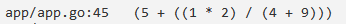
\includegraphics[width=0.7\textwidth]{parser/parserCodeResult.png}
	\caption{Результат работы синтаксического анализатора в виде строки}
	\label{f:parserCodeResult}
\end{figure}

Графическое представление AST для указанных входных данных представлено на рисунке~\ref{f:ast}.
Дерево, сформированное в результате работы программы для указанных входных данных представлен на рисунке~\ref{f:astRawCmd}.

\begin{figure}[ht]
	\centering
	\vspace{\toppaddingoffigure}
	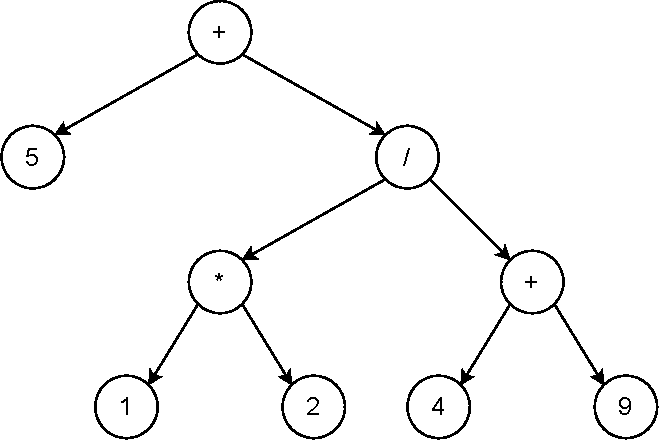
\includegraphics[width=0.7\textwidth]{parser/ast.pdf}
	\caption{AST для указанной входной строки}
	\label{f:ast}
\end{figure}

\clearpage

\begin{figure}[!htb]
	\centering
	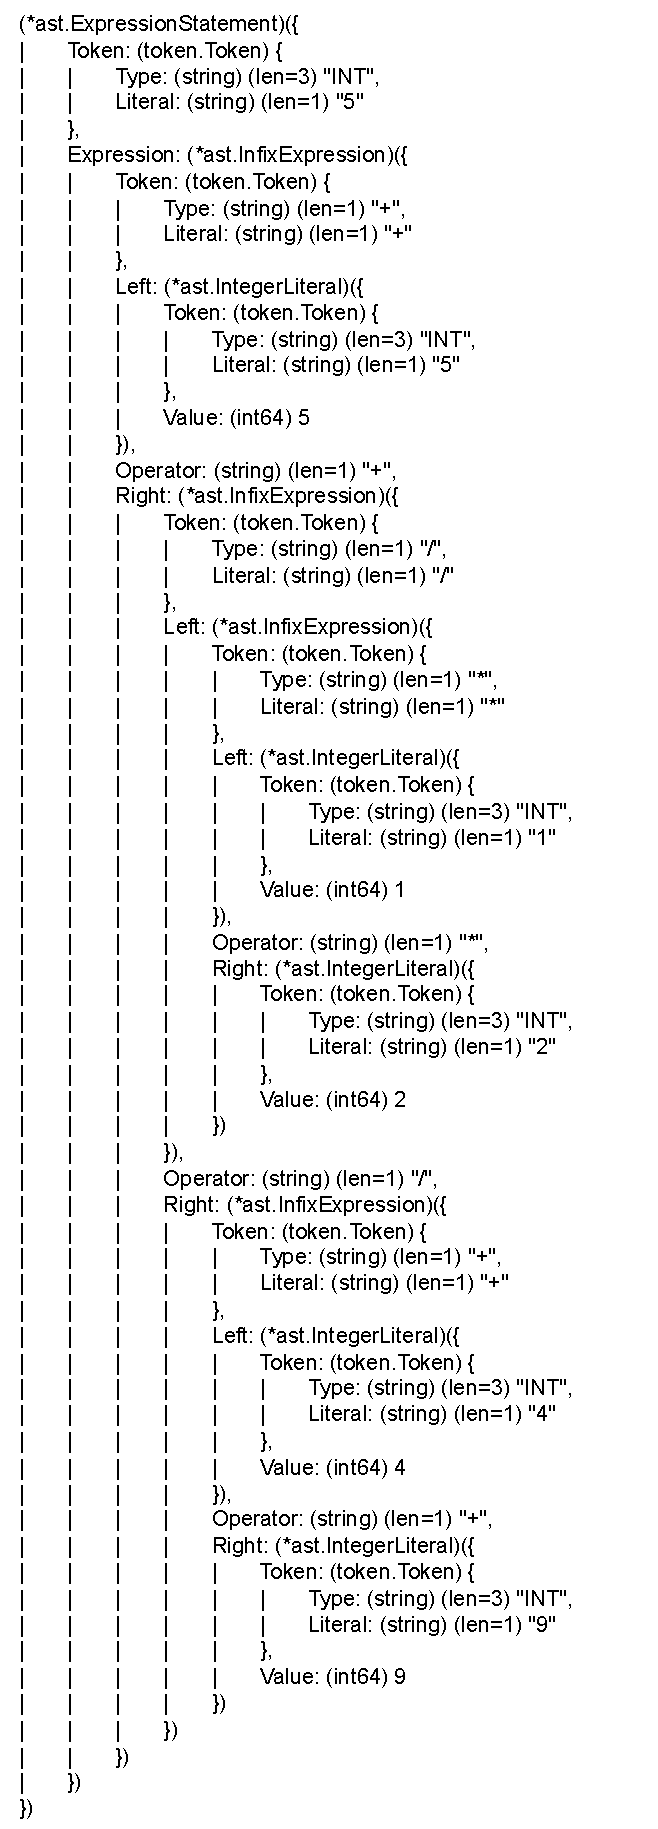
\includegraphics[width=0.48\textwidth]{parser/astRawCmd.pdf}
	\caption{Результат работы парсера в виде AST}
	\label{f:astRawCmd}
\end{figure}

\clearpage